\chapter{Clean Architecture}
Die Architektur der WebApi wurde nach den Regeln der Clean Architecture geplant. Dabei gibt es 5 Schichten die implementiert werden können. Diese Schichten sind in \ref{cleanArchitecture} zu sehen:
\begin{figure}[htbp]
    \centering
    \fbox{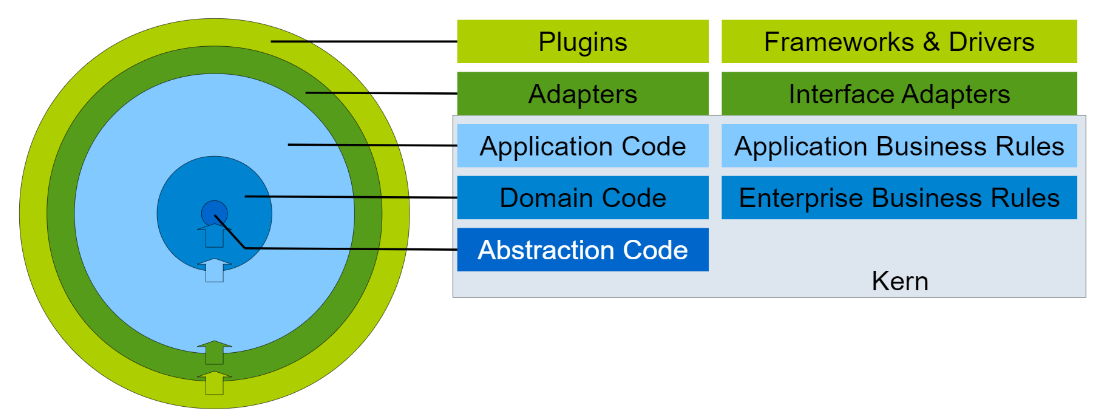
\includegraphics[width=10cm]{CleanArchitecture.png}}
    \caption{\label{cleanArchitecture} Schichten der Clean Architecture}
\end{figure}
Die Grundregeln der Clean Architecture besagen:
\begin{itemize}
    \item Der Anwendungs- und Domaincode ist frei von technischen Details
    \item Innere Schichten definieren Interfaces, äußere Schichten implementieren diese
    \item Sämtlicher Code kann eigenständig verändert werden
    \item Sämtlicher Code kann unabhängig von Infrastruktur kompiliert und ausgeführt werden
    \item Äußere Schichten koppeln sich an die inneren Schichten in richtung Zentrum
\end{itemize}
Hierbei ist die wichtigste aller Regeln, dass innere Schichten nicht von äußeren Schichten abhängen dürfen. Dadurch können äußere Schichten jederzeit ausgetauscht oder verädert werden, ohne dass die inneren Schichten etwas davon mitbekommen. 
Dies folgt auch dem Prinzip der Dependency Inversion.
\newline In diesem Projekt wurden 3 der 5 Schichten der Clean Architecture verwendet. Diese Schichten sind:
\begin{itemize}
    \item Plugin-Schicht
    \item Adapter-Schicht
    \item Domain-Schicht
\end{itemize}
Im Folgenden werden die verwendeten Schichten erklärt.
\section{Plugin-Schicht}
Die Plugin-Schicht ist die äußerste Schicht der Clean Architecture. Sie enthält die Klassen zum Starten der WebApi, stellt die Verbindung zur Datenbank her und führt Operationen auf der Datenbank aus.  
Außerdem liegen auf dieser Schicht die Controller, die die Anfragen entgegennehmen und Antworten zurück an den Client schicken.
\newline Sie implementiert die Repositories aus der Domain-Schicht und führt aufgrund dieser die Operationen auf der Datenbank aus. Die Adapter-Schicht wird verwendet , um die Ergebnisse aus der Datenbank umzumappen, 
damit sie an den Client zurückgeschickt werden können.  
\newline Die Plugin-Schicht ist die einzige Schicht, die externe Abhängigkeiten haben darf, da sie ganz außen liegt. In diesem Projekt ist dies beispielsweise 
durch die Abhängigkeit der Plugin-Schicht vom Entity Framework, das für die Datenbank-Operationen zuständig ist, zu sehen.
\section{Adapter-Schicht}
Die Adapter-Schicht konvertiert externe Formate so, dass die Applikation damit zurecht kommt und interne Formate so, dass externe Plugins damit zurecht kommen. Das Ziel dieser Struktur ist die Entkopplung von inneren und äußeren Schichten. Sie dient als Anti-Corruption Layer 
zwischen den Technischen Schichten und der Geschäftslogik.
\newline Da in diesem Programmentwurf mit einer InMemory-Datenbank, die innerhalb der Api läuft mit Hilfe der DbContext-Library und diese Einträge aufgrund der Entitäten der Anwendung baut, wird die Funktion externe Strukturen auf innere Strukturen abzubilden in der Adapter-Schicht nicht benötigt. 
Allerdings werden in der Adapter-Schicht in diesem Programmentwurf die interenen Strukturen wie Entitäten in Strukturen konvertiert, die an den Client weitergegeben werden können. Beispielsweise werden UserEntities in User-Objekte konvertiert, die nicht das Passwort des Benutzers enthalten, um eine Liste 
aller Benutzer in jedem Client darstellen zu können. Dadurch kann ein Benutzer alle anderen Benutzer sehen, um ihnen Geld zu überweisen, ohne dass der Client User-Objekte erhält, die das Passwort des Benutzers enthalten.
\section{Domain-Schicht}
In der Domain-Schicht befinden sich die Value Objects, Entities, Aggregates, Repositories und Domain Services. Die äußeren Schichten greifen auf diese Schicht zu, die Domain-Schicht kann aber auf keine andere Schicht zugreifen. Hier liegt die allgemeine Geschäftslogik. 
Dies hilft dabei zukünftig die Domain-Schicht auch in anderen Anwendungen verwenden zu können, wenn benötigt, da höchstens Abhängigkeiten von der Abstraction-Schicht bestehen, die sich nur sehr selten ändert. Die Repository-Interfaces, die in den äußeren Schichten implementiert werden, erlauben es der Domain-Schicht oder auch der Application-Schicht, wenn diese genutzt wird, auf die Datenbank zuzugreifen 
ohne von der Implementierung der Interfaces abhängig zu sein. Dadurch wird eine Inversion of Control erzeugt.
\newline Die Domain-Schicht in diesem Programmentwurf enthält alle der oben genannten Muster des Domain Driven Designs. 
\section{Weitere nicht implementierte Schichten}
\subsection{Application-Schicht}
In der Application-Schicht liegt die eigentliche anwendungsspezifische Geschäftslogik und die einzelnen Use Cases der Anwendung. Hier wird der Fluss der Daten von den Elementen der Domain-Schicht ausgehend und zu den Elementen führend gesteuert. 
Diese Schicht kann nur auf die Domain-Schicht zugreifen und Änderungen auf dieser Schicht beeinflussen die Domain-Schicht nicht. Sie funktioniert isoliert von Änderungen auf der Datenbank oder anderen Plugins, das bedeutet der genutzte Use Case weiß nicht, wer ihn aufgerufen hat oder auf 
welche Weise das Ergebnis präsentiert wird.
\newline Diese Schicht wurde in diesem Programmentwurf nicht explizit implementiert.
\subsection{Abstraction-Schicht}
Die Abstraction-Schicht enthält Domänen übergreifendes Wissen, wie Grundbausteine, die nicht domänenspezifisch sind, allgemeine Konzepte und Algorithmen oder nachgerüstete Libraries. Der Code auf dieser Schicht ändert sich selten bis nie und ist dadurch sehr stabil. Sie darf von keiner anderen Schicht abhängen, da 
sie nach dem Prinzip der Clean Architecture ganz innen liegt. In der Praxis muss diese Schicht häufig nicht explizit angelegt werden. Sie kann auch erst nachträglich eingebaut oder auch extrahiert werden. Genauere Beispiele für Code auf dieser Schicht sind beispielsweise Sortier-Algorithmen.
\newline Diese Schicht wurde in diesem Programmentwurf nicht explizit implementiert, da keine der zuvor genannten Bausteine oder Muster in dieser Anwendung verwendet werden.
